%%%%%%%%%%%%%%%%%%%%%%%%%%%%%%%%%%%%%%%%%%%%%%%%%%%%%%%%%%%%%%%%%%%%%
%% This is a (brief) model paper using the achemso class
%% The document class accepts keyval options, which should include
%% the target journal and optionally the manuscript type. 
%%%%%%%%%%%%%%%%%%%%%%%%%%%%%%%%%%%%%%%%%%%%%%%%%%%%%%%%%%%%%%%%%%%%%
\documentclass[journal=jacsat,manuscript=article]{achemso}

%%%%%%%%%%%%%%%%%%%%%%%%%%%%%%%%%%%%%%%%%%%%%%%%%%%%%%%%%%%%%%%%%%%%%
%% Place any additional packages needed here.  Only include packages
%% which are essential, to avoid problems later. Do NOT use any
%% packages which require e-TeX (for example etoolbox): the e-TeX
%% extensions are not currently available on the ACS conversion
%% servers.
%%%%%%%%%%%%%%%%%%%%%%%%%%%%%%%%%%%%%%%%%%%%%%%%%%%%%%%%%%%%%%%%%%%%%
\usepackage[version=4]{mhchem}
\usepackage{graphicx}
\usepackage{subcaption}
\captionsetup[subfigure]{labelfont=rm}
% \usepackage{subfigure}
%%%%%%%%%%%%%%%%%%%%%%%%%%%%%%%%%%%%%%%%%%%%%%%%%%%%%%%%%%%%%%%%%%%%%
%% If issues arise when submitting your manuscript, you may want to
%% un-comment the next line.  This provides information on the
%% version of every file you have used.
%%%%%%%%%%%%%%%%%%%%%%%%%%%%%%%%%%%%%%%%%%%%%%%%%%%%%%%%%%%%%%%%%%%%%
%%\listfiles

%%%%%%%%%%%%%%%%%%%%%%%%%%%%%%%%%%%%%%%%%%%%%%%%%%%%%%%%%%%%%%%%%%%%%
%% Place any additional macros here.  Please use \newcommand* where
%% possible, and avoid layout-changing macros (which are not used
%% when typesetting).
%%%%%%%%%%%%%%%%%%%%%%%%%%%%%%%%%%%%%%%%%%%%%%%%%%%%%%%%%%%%%%%%%%%%%
\newcommand*\mycommand[1]{\texttt{\emph{#1}}}

%%%%%%%%%%%%%%%%%%%%%%%%%%%%%%%%%%%%%%%%%%%%%%%%%%%%%%%%%%%%%%%%%%%%%
%% Meta-data block
%% ---------------
%% Each author should be given as a separate \author command.
%%
%% Corresponding authors should have an e-mail given after the author
%% name as an \email command. Phone and fax numbers can be given
%% using \phone and \fax, respectively; this information is optional.
%%
%% The affiliation of authors is given after the authors; each
%% \affiliation command applies to all preceding authors not already
%% assigned an affiliation.
%%
%% The affiliation takes an option argument for the short name.  This
%% will typically be something like "University of Somewhere".
%%
%% The \altaffiliation macro should be used for new address, etc.
%% On the other hand, \alsoaffiliation is used on a per author basis
%% when authors are associated with multiple institutions.
%%%%%%%%%%%%%%%%%%%%%%%%%%%%%%%%%%%%%%%%%%%%%%%%%%%%%%%%%%%%%%%%%%%%%
\author{Nianhan Tian}
\affiliation[Georgia Institute of Technology]
{School of Chemical and Biomolecular Engineering, Georgia Institute of Technology, Atlanta, Georgia 30318 USA}

\author{Andrew J. Medford}
\affiliation[Georgia Institute of Technology]
{School of Chemical and Biomolecular Engineering, Georgia Institute of Technology, Atlanta, Georgia 30318 USA}
\email{ajm@gatech.edu}
%%%%%%%%%%%%%%%%%%%%%%%%%%%%%%%%%%%%%%%%%%%%%%%%%%%%%%%%%%%%%%%%%%%%%
%% The document title should be given as usual. Some journals require
%% a running title from the author: this should be supplied as an
%% optional argument to \title.
%%%%%%%%%%%%%%%%%%%%%%%%%%%%%%%%%%%%%%%%%%%%%%%%%%%%%%%%%%%%%%%%%%%%%
% \title[An \textsf{achemso} demo]
\title{Accelerated Computational Materials Discovery for Electrochemical Nutrient Recovery}

%%%%%%%%%%%%%%%%%%%%%%%%%%%%%%%%%%%%%%%%%%%%%%%%%%%%%%%%%%%%%%%%%%%%%
%% Some journals require a list of abbreviations or keywords to be
%% supplied. These should be set up here, and will be printed after
%% the title and author information, if needed.
%%%%%%%%%%%%%%%%%%%%%%%%%%%%%%%%%%%%%%%%%%%%%%%%%%%%%%%%%%%%%%%%%%%%%
\abbreviations{IR,NMR,UV}
\keywords{American Chemical Society, \LaTeX}

%%%%%%%%%%%%%%%%%%%%%%%%%%%%%%%%%%%%%%%%%%%%%%%%%%%%%%%%%%%%%%%%%%%%%
%% The manuscript does not need to include \maketitle, which is
%% executed automatically.
%%%%%%%%%%%%%%%%%%%%%%%%%%%%%%%%%%%%%%%%%%%%%%%%%%%%%%%%%%%%%%%%%%%%%
\begin{document}


%%%%%%%%%%%%%%%%%%%%%%%%%%%%%%%%%%%%%%%%%%%%%%%%%%%%%%%%%%%%%%%%%%%%%
%% The abstract environment will automatically gobble the contents
%% if an abstract is not used by the target journal.
%%%%%%%%%%%%%%%%%%%%%%%%%%%%%%%%%%%%%%%%%%%%%%%%%%%%%%%%%%%%%%%%%%%%%
\begin{abstract}
 
\end{abstract}

%%%%%%%%%%%%%%%%%%%%%%%%%%%%%%%%%%%%%%%%%%%%%%%%%%%%%%%%%%%%%%%%%%%%%
%% Start the main part of the manuscript here.
%%%%%%%%%%%%%%%%%%%%%%%%%%%%%%%%%%%%%%%%%%%%%%%%%%%%%%%%%%%%%%%%%%%%%
\section{Introduction}

% Problem statement 
% Growing global interest in sustainable methods for nutrient recovery from wastewater.
% Challenges in identifying materials that are stable and efficient under experimental electrochemical conditions.

% Background for electrochemical nutrient recovery.

Traditionally, nitrogen-based fertilizers are produced from ammonia by the Haber-Bosch process \cite{Schloegl2003CatalyticStory}. The Haber-Bosch process operates under [insert] temperatures and pressures, leaving a significant carbon footprint \cite{Liu2022ProspectsFixation, Smil1999DetonatorExplosion,Suryanto2021NitrogenShuttle}. In contrast, organic waste from sewage and farms offers an alternative resource for nutrient recovery, particularly nitrogen, which constitutes 30–40\% of waste sludge in the form of proteins [insert reference]. Electrochemical methods, such as the electrolysis of waste-activated sludge, provide an alternative for recovering nitrogen while reducing environmental impact. However, the development of efficient and stable catalysts for electrochemical waste sludge oxidation remains a significant challenge. 

% Importance of Stability in Materials Discovery
% Stability as a critical factor for long-term performance in electrochemical systems.
% How Pourbaix diagrams provide thermodynamic insights into stability.

Despite ongoing efforts in electrochemical nutrient recovery, the identification of active, selective, and stable materials for this application has faced challenges due to a lack of comprehensive computational and experimental studies. One of the primary challenges lies in the stability of the catalyst material under high-voltage and nitrogen-rich aqueous environments. Electrodes often suffer from dissolution and corrosion [insert citation], which compromise their performance. Addressing these stability issues is crucial for enabling sustainable electrochemical nutrient recovery processes.

% 1.3 Inspiration from Hydrometallurgy
% Role of nitrogen-containing ligands in hydrometallurgical processes.
% Difference in nitrogen concentration conditions between hydrometallurgy and electrochemical recovery.

The thermodynamic stability of materials under electrochemical conditions can be described by Pourbaix diagrams \cite{PourbaixAtlasSolutions}. Pourbaix diagrams demonstrate the relative stable regions of solid bulk species and solvated aqueous ions as a function of applied potential and pH. These diagrams help identify the effect of electrochemical experimental parameters on material's phase stability [insert citation]. In corrosion studies, Pourbaix diagrams are used to identify optimal applied potentials and pH such that electrodes are stable and will not dissolve. These diagrams also help find passitating regions where bulk metals can form a metal oxide layer that prevents further surface attack by oxygen in the solution, or induced by oxidizing potentials. Most available Pourbaix diagram studies of electrochemical system only account for the affect of the ionic activity of hydrogen, so the stability of bulk materials under these conditions cannot be directly used to identify stable regions of electrode under high nitrogen containing ligand concentrations. In hydrometallurgy studies, Pourbaix diamgrams are used to identify optimal conditions for metal leaching to recover rare or toxic metals from ores. Recent work has extended these diagrams to metal leaching induced by nitrogen-containing ligands such as ammonia\cite{Meng1996PrinciplesReview}, glycine and cyanide. Although these studies are typically conducted under conditions of high temperature and high leaching solution concentration, which differ significantly from those relevant to electrochemical nutrient recovery, Pourbaix diagrams that cover the effect of N-containing ligands can be used to identify electrode stability and accelerate catalyst design by focusing on stable compositions. 

We also want to avoid electrode dissolution so that the electrochemical oxidation is sustainable and fertilizers end-product are non-toxic. 
% 1.4 Objective and Scope of the Study
% Propose a stability-based computational framework using Pourbaix diagrams.
% Outline the focus on nitrogen-rich environments for electrochemical nutrient recovery.

In this study, we adapt the Pourbaix diagram approach to experimental conditions specific to electrochemical waste sludge oxidation, focusing on the potential and pH ranges pertinent to nutrient recovery. By generating and analyzing Pourbaix diagrams under these conditions, we aim to establish a computational framework for screening materials based on stability—a criterion often overlooked in favor of activity and selectivity. This framework emphasizes the importance of stability as a foundational parameter for identifying optimal catalysts for electrochemical nutrient recovery.

Through this work, we present a material screening strategy that integrates stability, activity, and selectivity to identify materials capable of efficient and selective nitrogen recovery from organic waste. By leveraging computational insights and thermodynamic stability analysis, this study provides a pathway toward designing robust and sustainable catalysts for electrochemical nutrient recovery.


\section{Methods}
\subsection{Pourbaix Diagram Construction}
Pourbaix diagrams were constructed to map the thermodynamic stability regions of bulk metals and their metal-ligand complexes under electrolysis of waste activated sludge (EWAS) potentials in basic environment. Free energies of bulk metals were obtained from the Materials Project database \cite{Jain2013TheInnovation}, based on generalized gradient approximation (GGA) density functional theory (DFT) calculations. Free energies for aqueous ligands and metal-ligand complexes were calculated from equilibrium constants sourced from standard thermochemical handbooks \cite{MartellCriticalSupplement, Smith1976CriticalConstants, Bard2017StandardSolution} and literatures \cite{Meng1996PrinciplesReview, Azadi2019DataComplexes, Aviles2022ExploringNH3, Oraby2023SelectiveSolutions}. Metal elements that are traditionally used as electrode materials are considered in this study, including Au, Cu, Ni, Co, Mg, Mn, Ti, Zn, Ag, Cd, Sr, Pt, Pd and Fe. The aqueous ligands considered in this study include \ce{NH3-}, glycine and \ce{CN-}. The targeted experimental potential ranges from -2.0-2.3 V (vs RHE) and the pH ranges from 11.5-13.5.

\begin{equation} \label{eq:reaction}
aA + h\text{H}^+ + z\text{e}^- \leftrightarrow bB + \text{H}_2\text{O}
\end{equation}

The diagrams were constructed based the framework introduced by previous studies \cite{PourbaixAtlasSolutions, Huang2017ImprovedCompounds, Huang2015ElectrochemicalCalculations,Singh2017ElectrochemicalMaterials,Patel2019EfficientCompounds,Persson2012PredictionStates}. All reaction species, i.e. metal, oxides, aqueous ions and ligands, and water are connected by corresponding reactions. Then the reaction chemical potentials are derived from equilibrium relationships between species, using the Nernst equations, as a function of applied potential and pH. For a redox reaction shown in Equation~\eqref{eq:reaction}, the Nernst equation is:

\begin{equation} \label{eq:nernst} E = E^\circ - \frac{k}{z} \log \left(\frac{A^a}{B^b}\right) - \frac{k \cdot h}{z} \text{pH}, \end{equation}

where \(E\) is the cell potential at non-standard conditions, \(E^\circ\) is the standard electrode potential, and k is defined as \(k = \frac{RT}{F} \cdot \frac{1}{\ln 10}\). \(A\) and \(B\) are the activities of the reactants and products, and \(z\) is the number of electrons transferred. \(a\), \(b\) and \(h\) are the stroichiometric coefficients of reactants, products, and protons, respectively. Aqueous ion activities are assumed to be 10$^-4$ M. Ligand concentrations are set according to experimental conditions. 

The Pourbaix diagrams were generated by evaluating the chemical potentials of all species across a finely spaced potential-pH grid (4000 $\times$ 4000 points) and identifying the most thermodynamically stable species at each grid point. The thermodynamic stability of each species was calculated by comparing chemical potentials at each grid point across the potential-pH space. Stability regions were identified for bulk metals, aqueous ions, and metal-ligand complexes. 


\subsection{Incorporation of Nitrogen Ligands}
To extend the Pourbaix framework to systems containing nitrogen-based ligands (\ce{NH3}, glycine, and \ce{CN-}), ligand concentrations are represented as pligand in Equation~\eqref{eq:pligand} and incorporated into pH-dependent mass balance equations, assuming that the sum of the concentrations of protonated and deprotonated spcies is kept constant. For example, the dissociation equilibrium of \ce{NH3} (Equation~\eqref{eq:NH3 equilibrium}) indicates the relationship between pH and p\ce{NH3} via Equation~\eqref{eq:pNH3}:

\begin{equation} \label{eq:NH3 equilibrium}
\ce{NH4+} \leftrightarrow \ce{NH3} + \ce{H+}
\end{equation}
% \begin{equation} \label{eq:NH3_total}
% [\text{NH}_3]_{\text{total}} = [\text{NH}_3] + [\text{NH}_4^+]
% \end{equation}
\begin{equation} \label{eq:pNH3}
\text{pNH}_3 = -\log \left([\text{NH}_3]_{\text{tot}}\right) + \log \left(1 + 10^{pK_a - pH} \right), \quad pK_a = 9.26 \cite{NationalCenterforBiotechnologyInformation2025PubChemHSDB}
\end{equation}

Similarly, glycine and \ce{CN-} concentrations were calculated using Equations~\eqref{eq:pGly} and~\eqref{eq:pCN}, respectively:
\begin{align} \label{eq:pGly}
\text{pGly} &= -\log \left([\text{Gly}_{\text{total}}]\right) + (pK_{a_1} - pH) \nonumber \\
&\quad + \log \left(1 + 10^{pH - pK_{a_1}} + \frac{1}{10^{pH - pK_{a_2}}} \right), \nonumber \\
&\quad pK_{a_1} = 2.37, \quad pK_{a_2} = 9.8 \cite{2025PubChemGlycine.}
\end{align}
\begin{equation} \label{eq:pCN}
\text{pCN}^- = -\log \left([\text{CN}^-]_{\text{tot}}\right) + \log \left(1 + 10^{pK_a - pH} \right), \quad pK_a = 9.2 \cite{USEPA1980AmbientCyanides}
\end{equation}
\begin{equation} \label{eq:pligand}
\text{pligand} = -\log[\text{ligand}].
\end{equation}

The interdependence of pH and ligand concentration (e.g., due to \ce{NH3} equilibrium in Equation~\eqref{eq:NH3 equilibrium}) was explicitly modeled. It was further assumed that ligand concentrations were unaffected by other ligands or external factors. For example, when both \ce{NH3} and \ce{CN-} were present, their equilibrium concentrations were treated as independent functions of pH.



\section{Results and discussion}
The constructed Pourbaix diagrams are shown in Figure 

A pourbaix diagram of the xxx system with tot concentration of xxxx M is shown inxxx. Ammine complaxed with ions with xx number of coordinated ammonia is known to form xxx. 


The Pourbaix diagram of Ni-\ce{NH3}-Gly-\ce{H2O} and Ni-\ce{H2O} is shown in Fig. \ref{Ni Pourbaix diagram}. From the comparison, we can see that the addition of N-ligands significantly affects the stability of Ni bulk species and aqueous species. N-ligands can form Ni-ligand complexes that have more stable thermodynamic free energies than some bulk species, therefore changing the stability domains of solid Ni oxides. The intended experimental conditions for the current experiments is bounded by the green box in Fig.\ref{Ni Pourbaix diagram}. We can see that the bulk Ni electrode is likely to be complexed by Gly ligand under the experimental condition, since the metal-ligand complex is more thermodynamically stability than other species and can form over the intended experimental conditions. The stable regions of Ni's metal-ligands complexes over the range of applied potential and pH partially explain Ni's dissolvation under oxidizing potential and high ammonia concentration observed in experiments from a thermodynamics perspective, although a more thorough kinetics study should be performed to determine if the thermodynamics free energy is the main driving force of dissolution. 

The Pourbaix diagram of other common metals that can be used as electrode in electrochemistry experiments are shown in Figs. x to x. From a thermodynamics perspective, these metal can all complex with N-ligands under intended experimental conditions, besides Ti. 
\begin{figure}[htbp]
    \centering
    % Subfigure (a)
    \begin{subfigure}[b]{0.3\textwidth}
        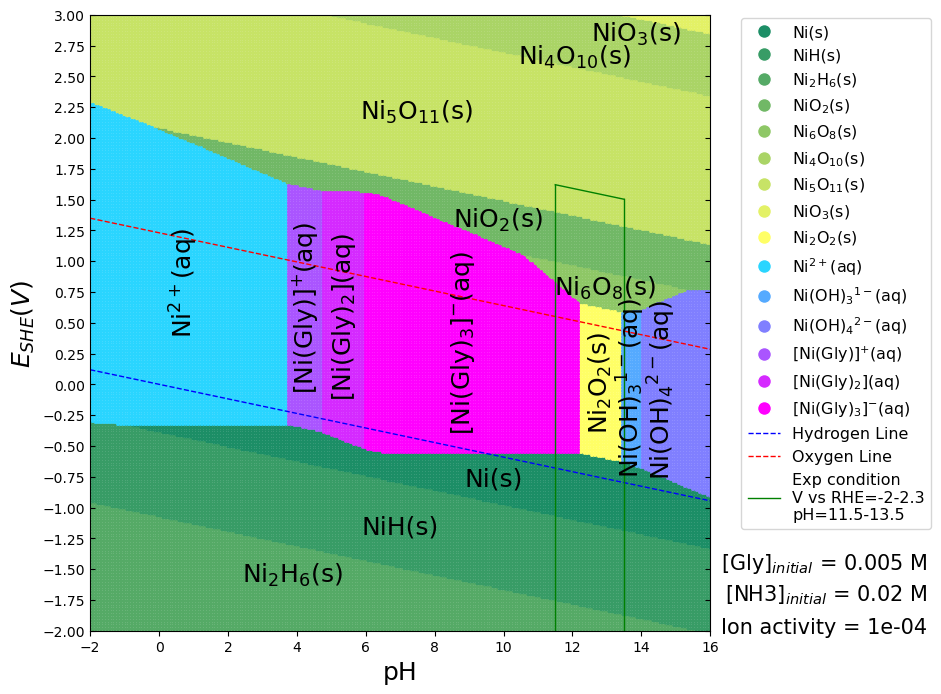
\includegraphics[width=\textwidth]{Figures/pourbaix_diagrams/Ni-NH3-H2O_activity=1e-04_[NH3]=0.02M_[Gly]=0.005M_[CN]=0.png}
        \caption{}\label{fig:Ni_Pourbaix}
        \par\medskip
    \end{subfigure}
    % Subfigure (b)
    \begin{subfigure}[b]{0.3\textwidth}
        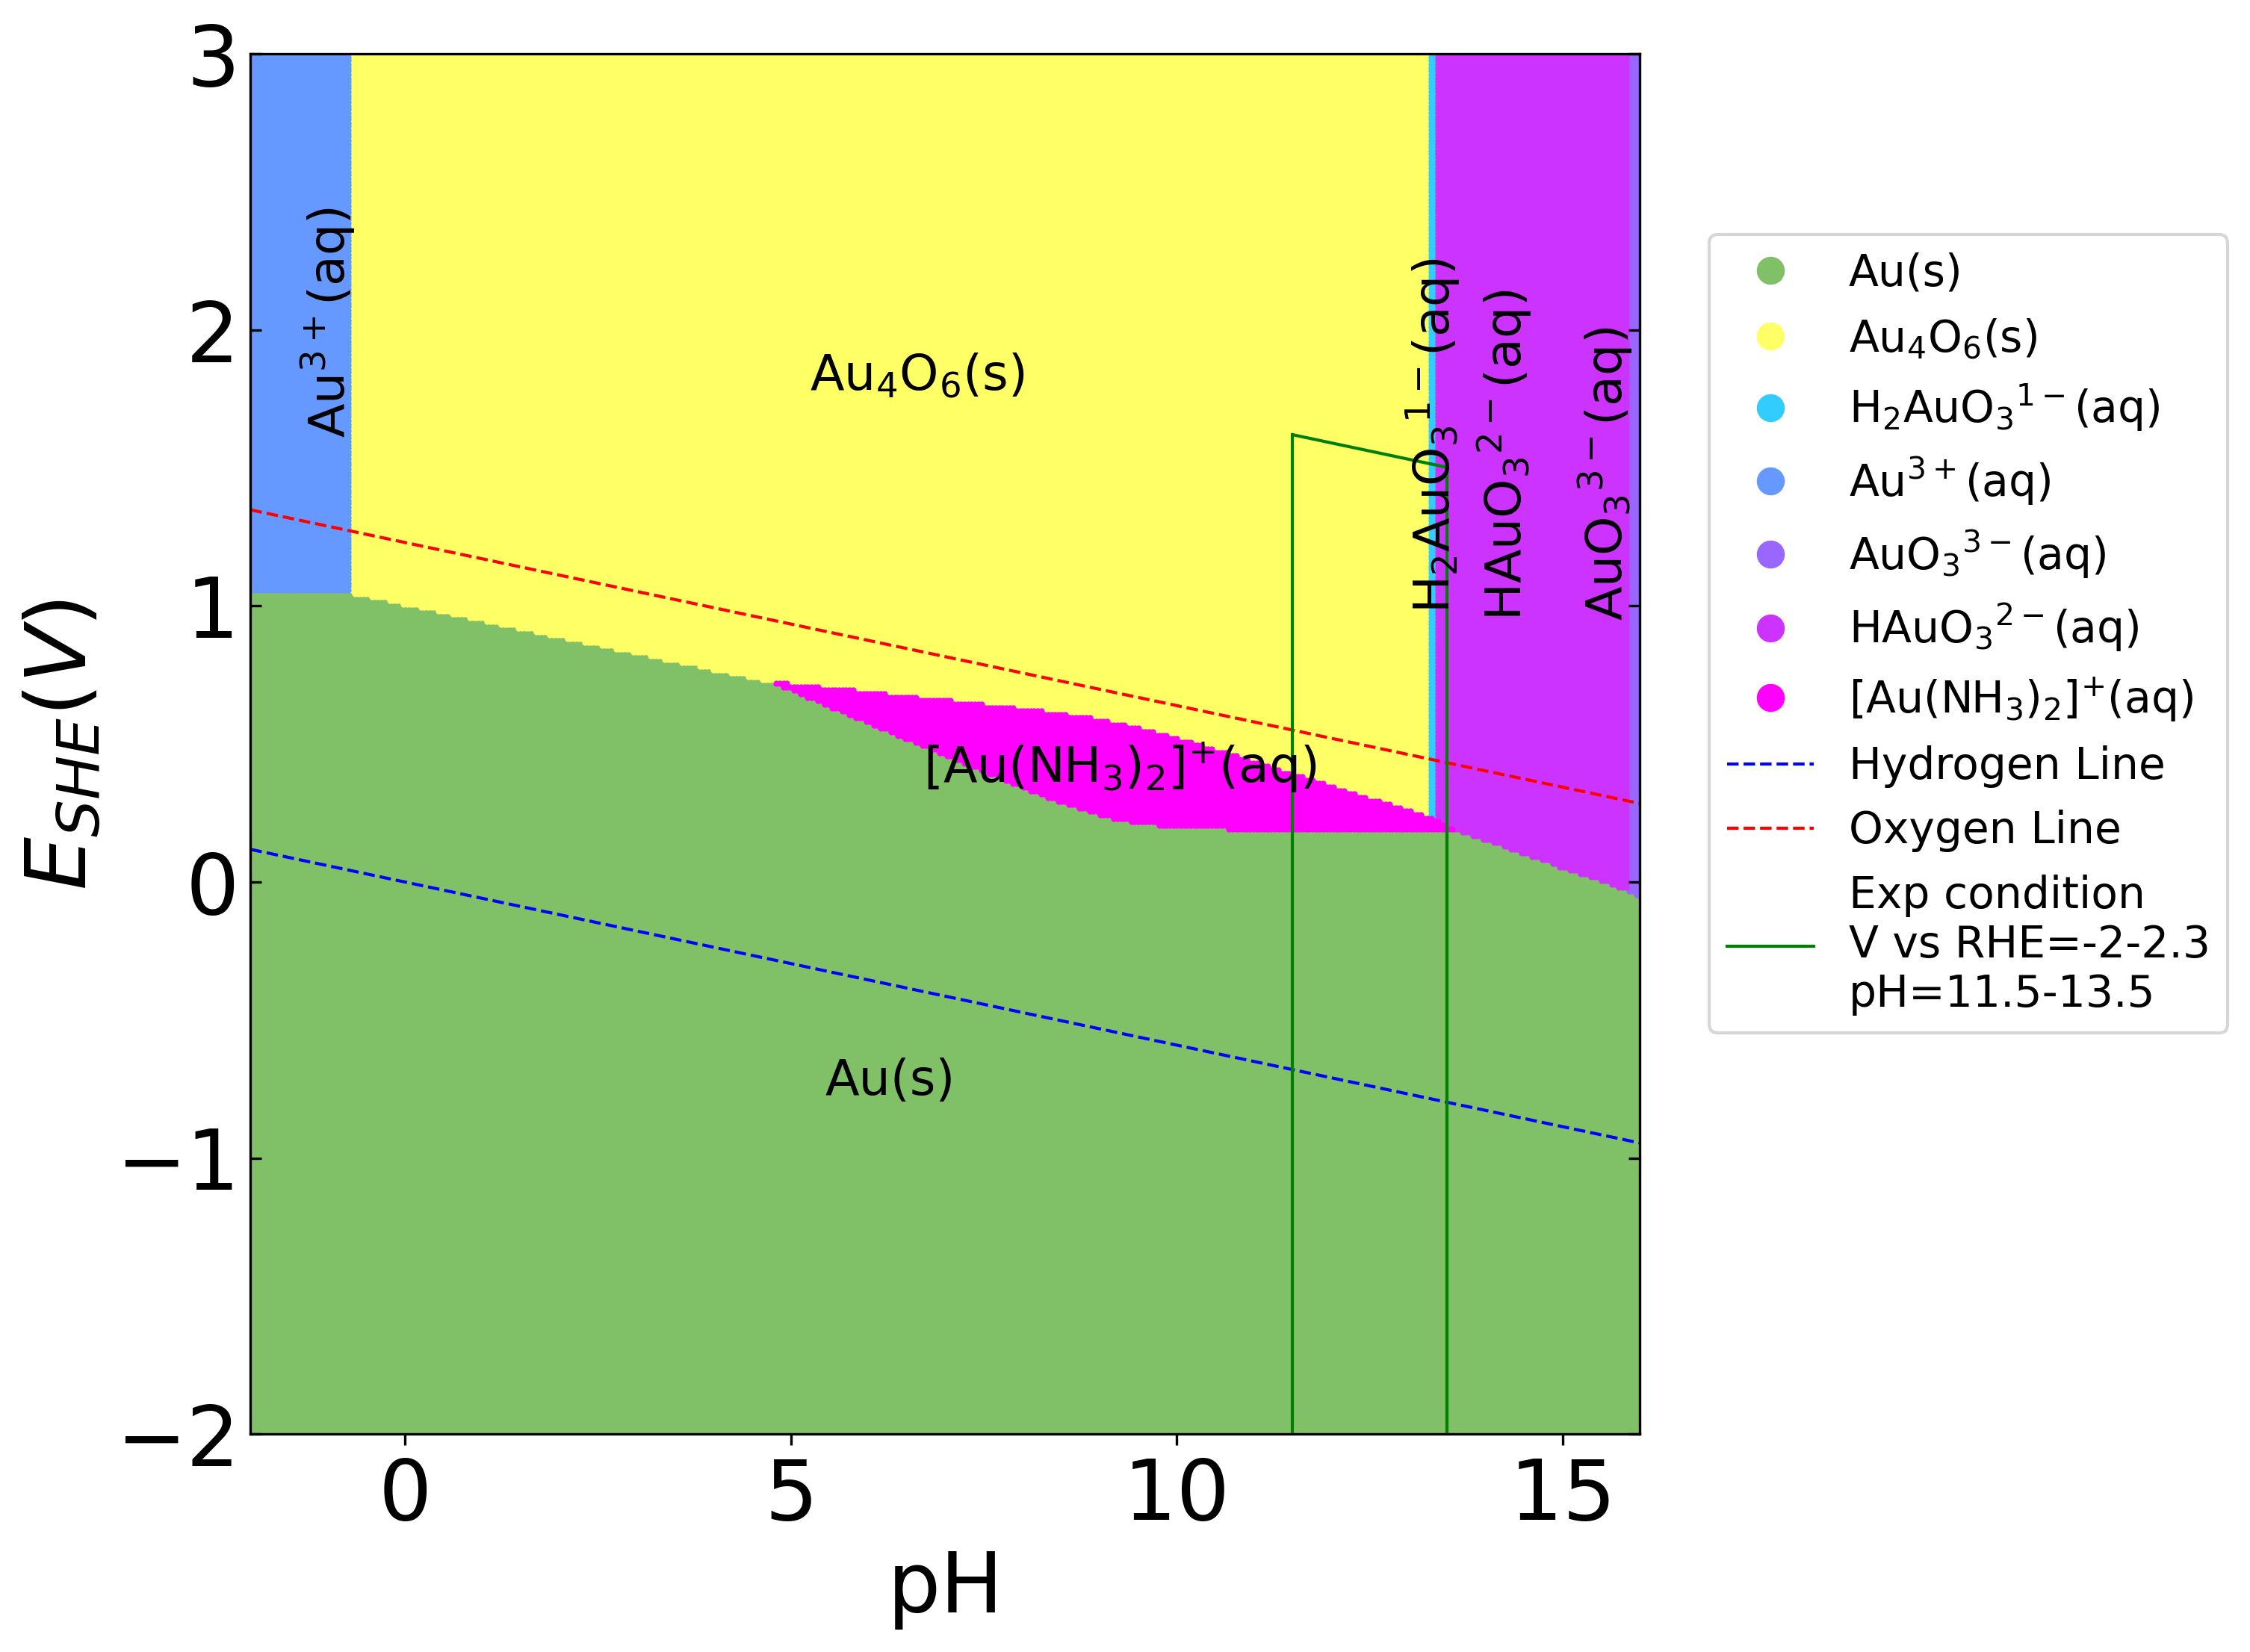
\includegraphics[width=\textwidth]{Figures/pourbaix_diagrams/Au-NH3-H2O_activity=1e-04_[NH3]=0.02M_[Gly]=0.005M_[CN]=0.png}
        \caption{}\label{fig:Au_Pourbaix}
        \par\medskip
    \end{subfigure}
    % Subfigure (c)
    \begin{subfigure}[b]{0.3\textwidth}
        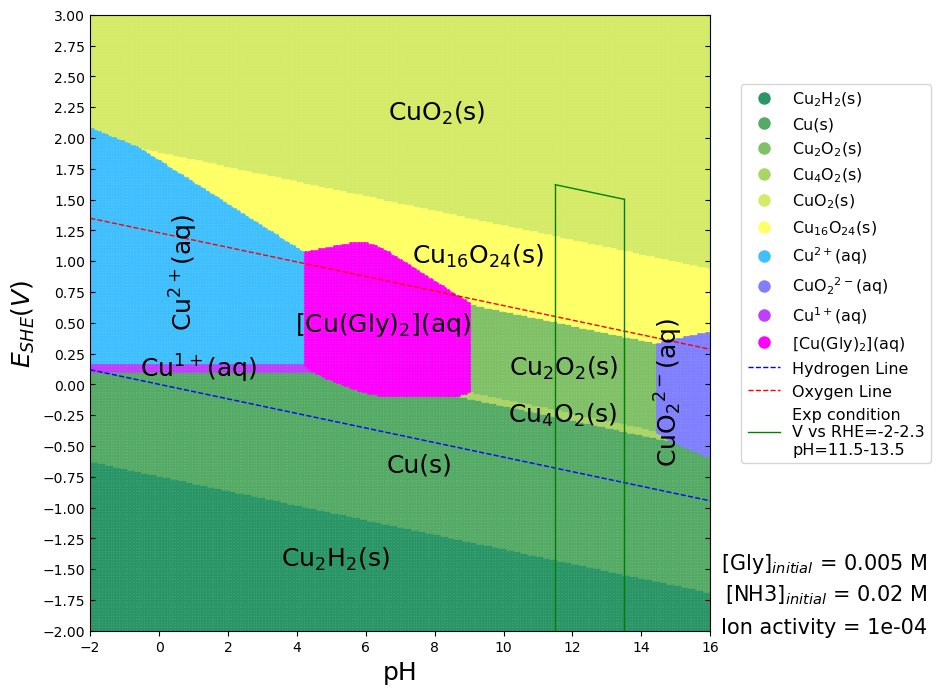
\includegraphics[width=\textwidth]{Figures/pourbaix_diagrams/Cu-NH3-H2O_activity=1e-04_[NH3]=0.02M_[Gly]=0.005M_[CN]=0.png}
        \caption{}\label{fig:Cu_Pourbaix}
        \par\medskip
        
    \end{subfigure}
    % Subfigure (d)
    \begin{subfigure}[b]{0.3\textwidth}
        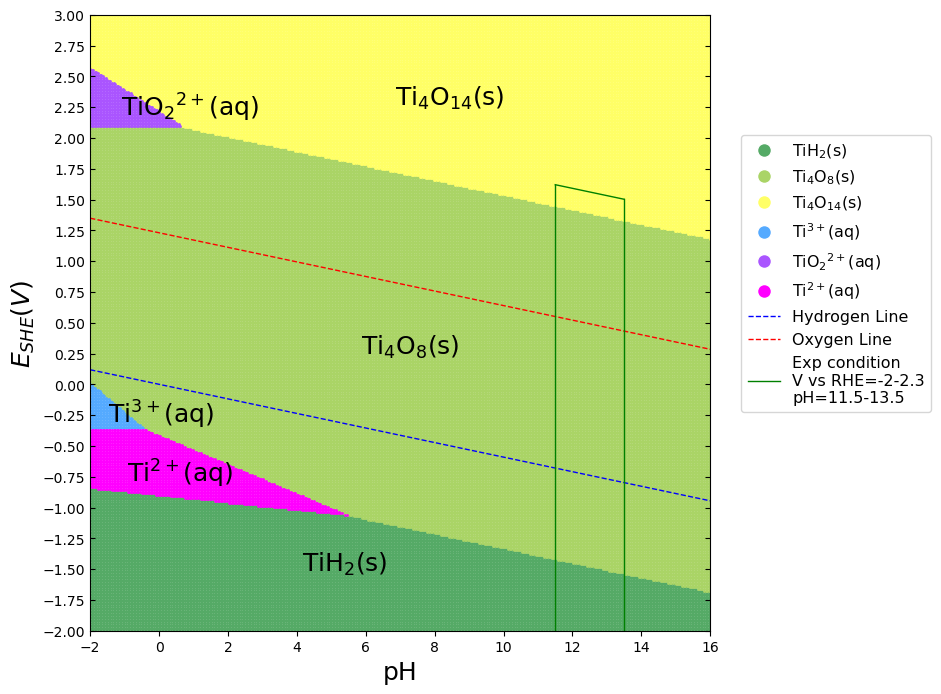
\includegraphics[width=\textwidth]{Figures/pourbaix_diagrams/Ti-NH3-H2O_activity=1e-04_[NH3]=0.02M_[Gly]=0.005M_[CN]=0.png}
        \caption{}\label{fig:Ti_Pourbaix}
    \end{subfigure}
    % Subfigure (e)
    \begin{subfigure}[b]{0.3\textwidth}
        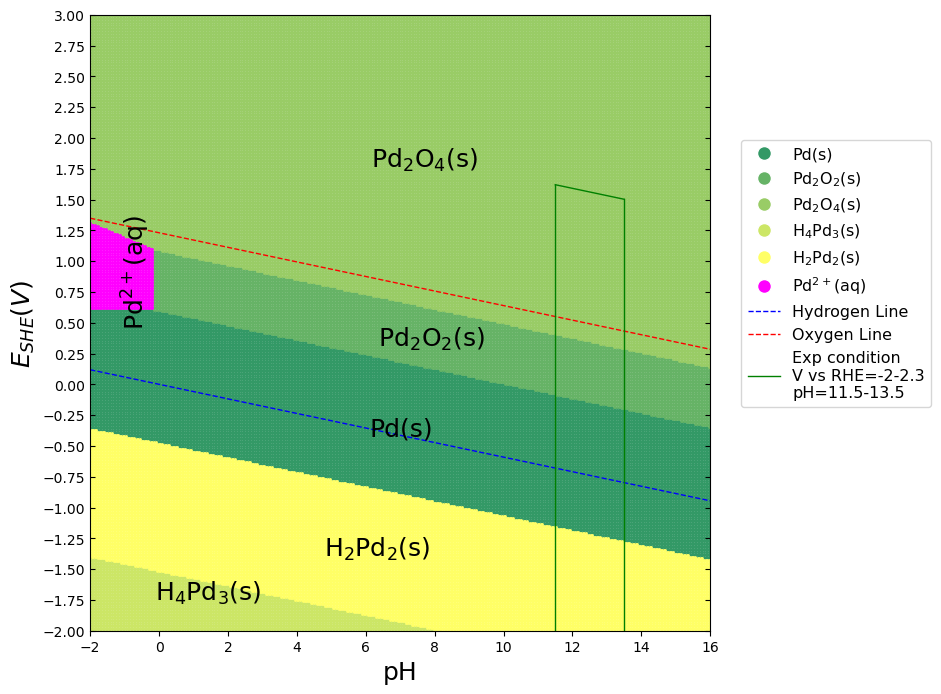
\includegraphics[width=\textwidth]{Figures/pourbaix_diagrams/Pd-NH3-H2O_activity=1e-04_[NH3]=0.02M_[Gly]=0.005M_[CN]=0.png}
        \caption{}\label{fig:Pd_Pourbaix}
    \end{subfigure}
    % Subfigure (f)
    \begin{subfigure}[b]{0.3\textwidth}
        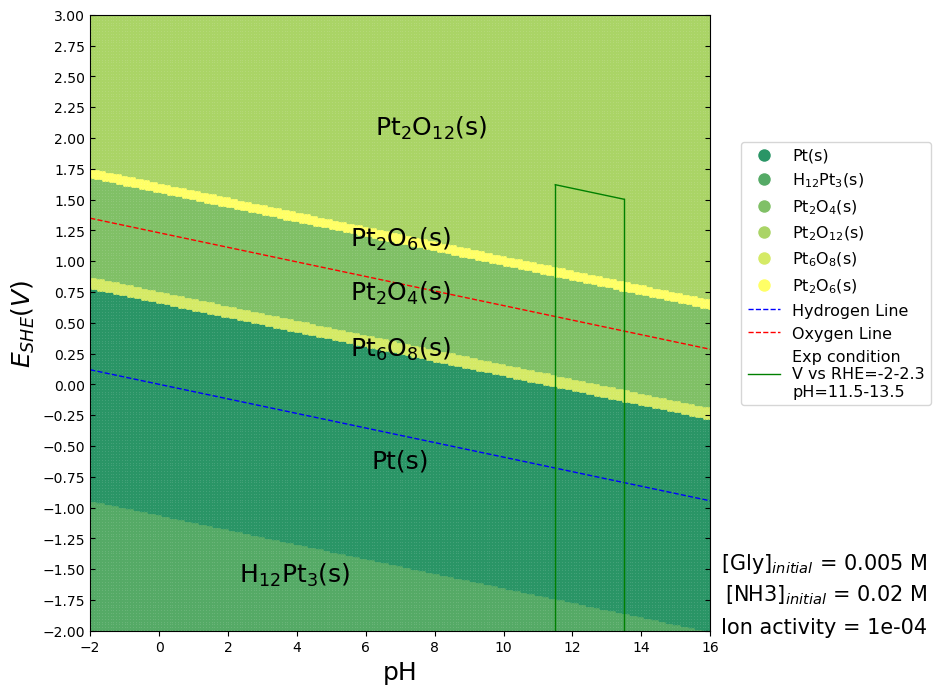
\includegraphics[width=\textwidth]{Figures/pourbaix_diagrams/Pt-NH3-H2O_activity=1e-04_[NH3]=0.02M_[Gly]=0.005M_[CN]=0.png}
        \caption{}\label{fig:Pt_Pourbaix}
    \end{subfigure}

    \caption{Pourbaix diagrams for different metals at $[NH_3]_{initial}= 0.02M$, $[Gly]_{initial}=0.005M$. Green box indicates experimental condition at applied potential vs RHE = -2 to 2 V, pH = 11.5 to 13.5.}
    \label{fig:Pourbaix_all}
\end{figure}

% \begin{figure}
% 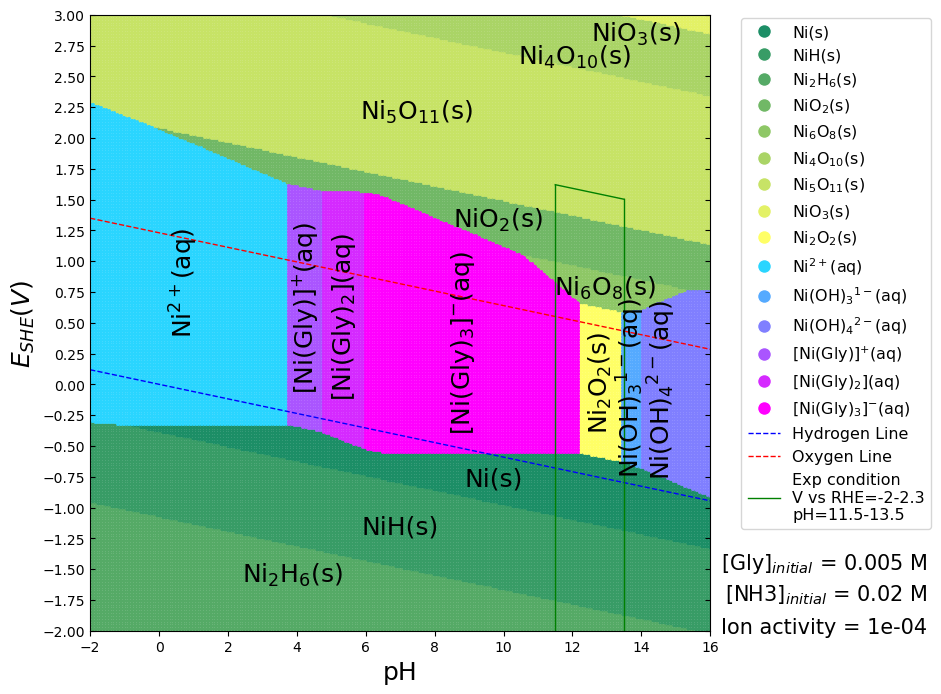
\includegraphics[width=0.5\textwidth]{Figures/pourbaix_diagrams/Ni-NH3-H2O_activity=1e-04_[NH3]=0.02M_[Gly]=0.005M_[CN]=0.png}
%   \caption{Ni Pourbaix diagram at $[NH_3]_{initial}= 0.02M$, $[Gly]_{initial}=0.005M$. Green box indicates experimental condition at applied potential vs RHE = -2 to 2 V, pH =11.5 to 13.5}
%   \label{Ni Pourbaix diagram}
% \end{figure}

% \begin{figure}
% 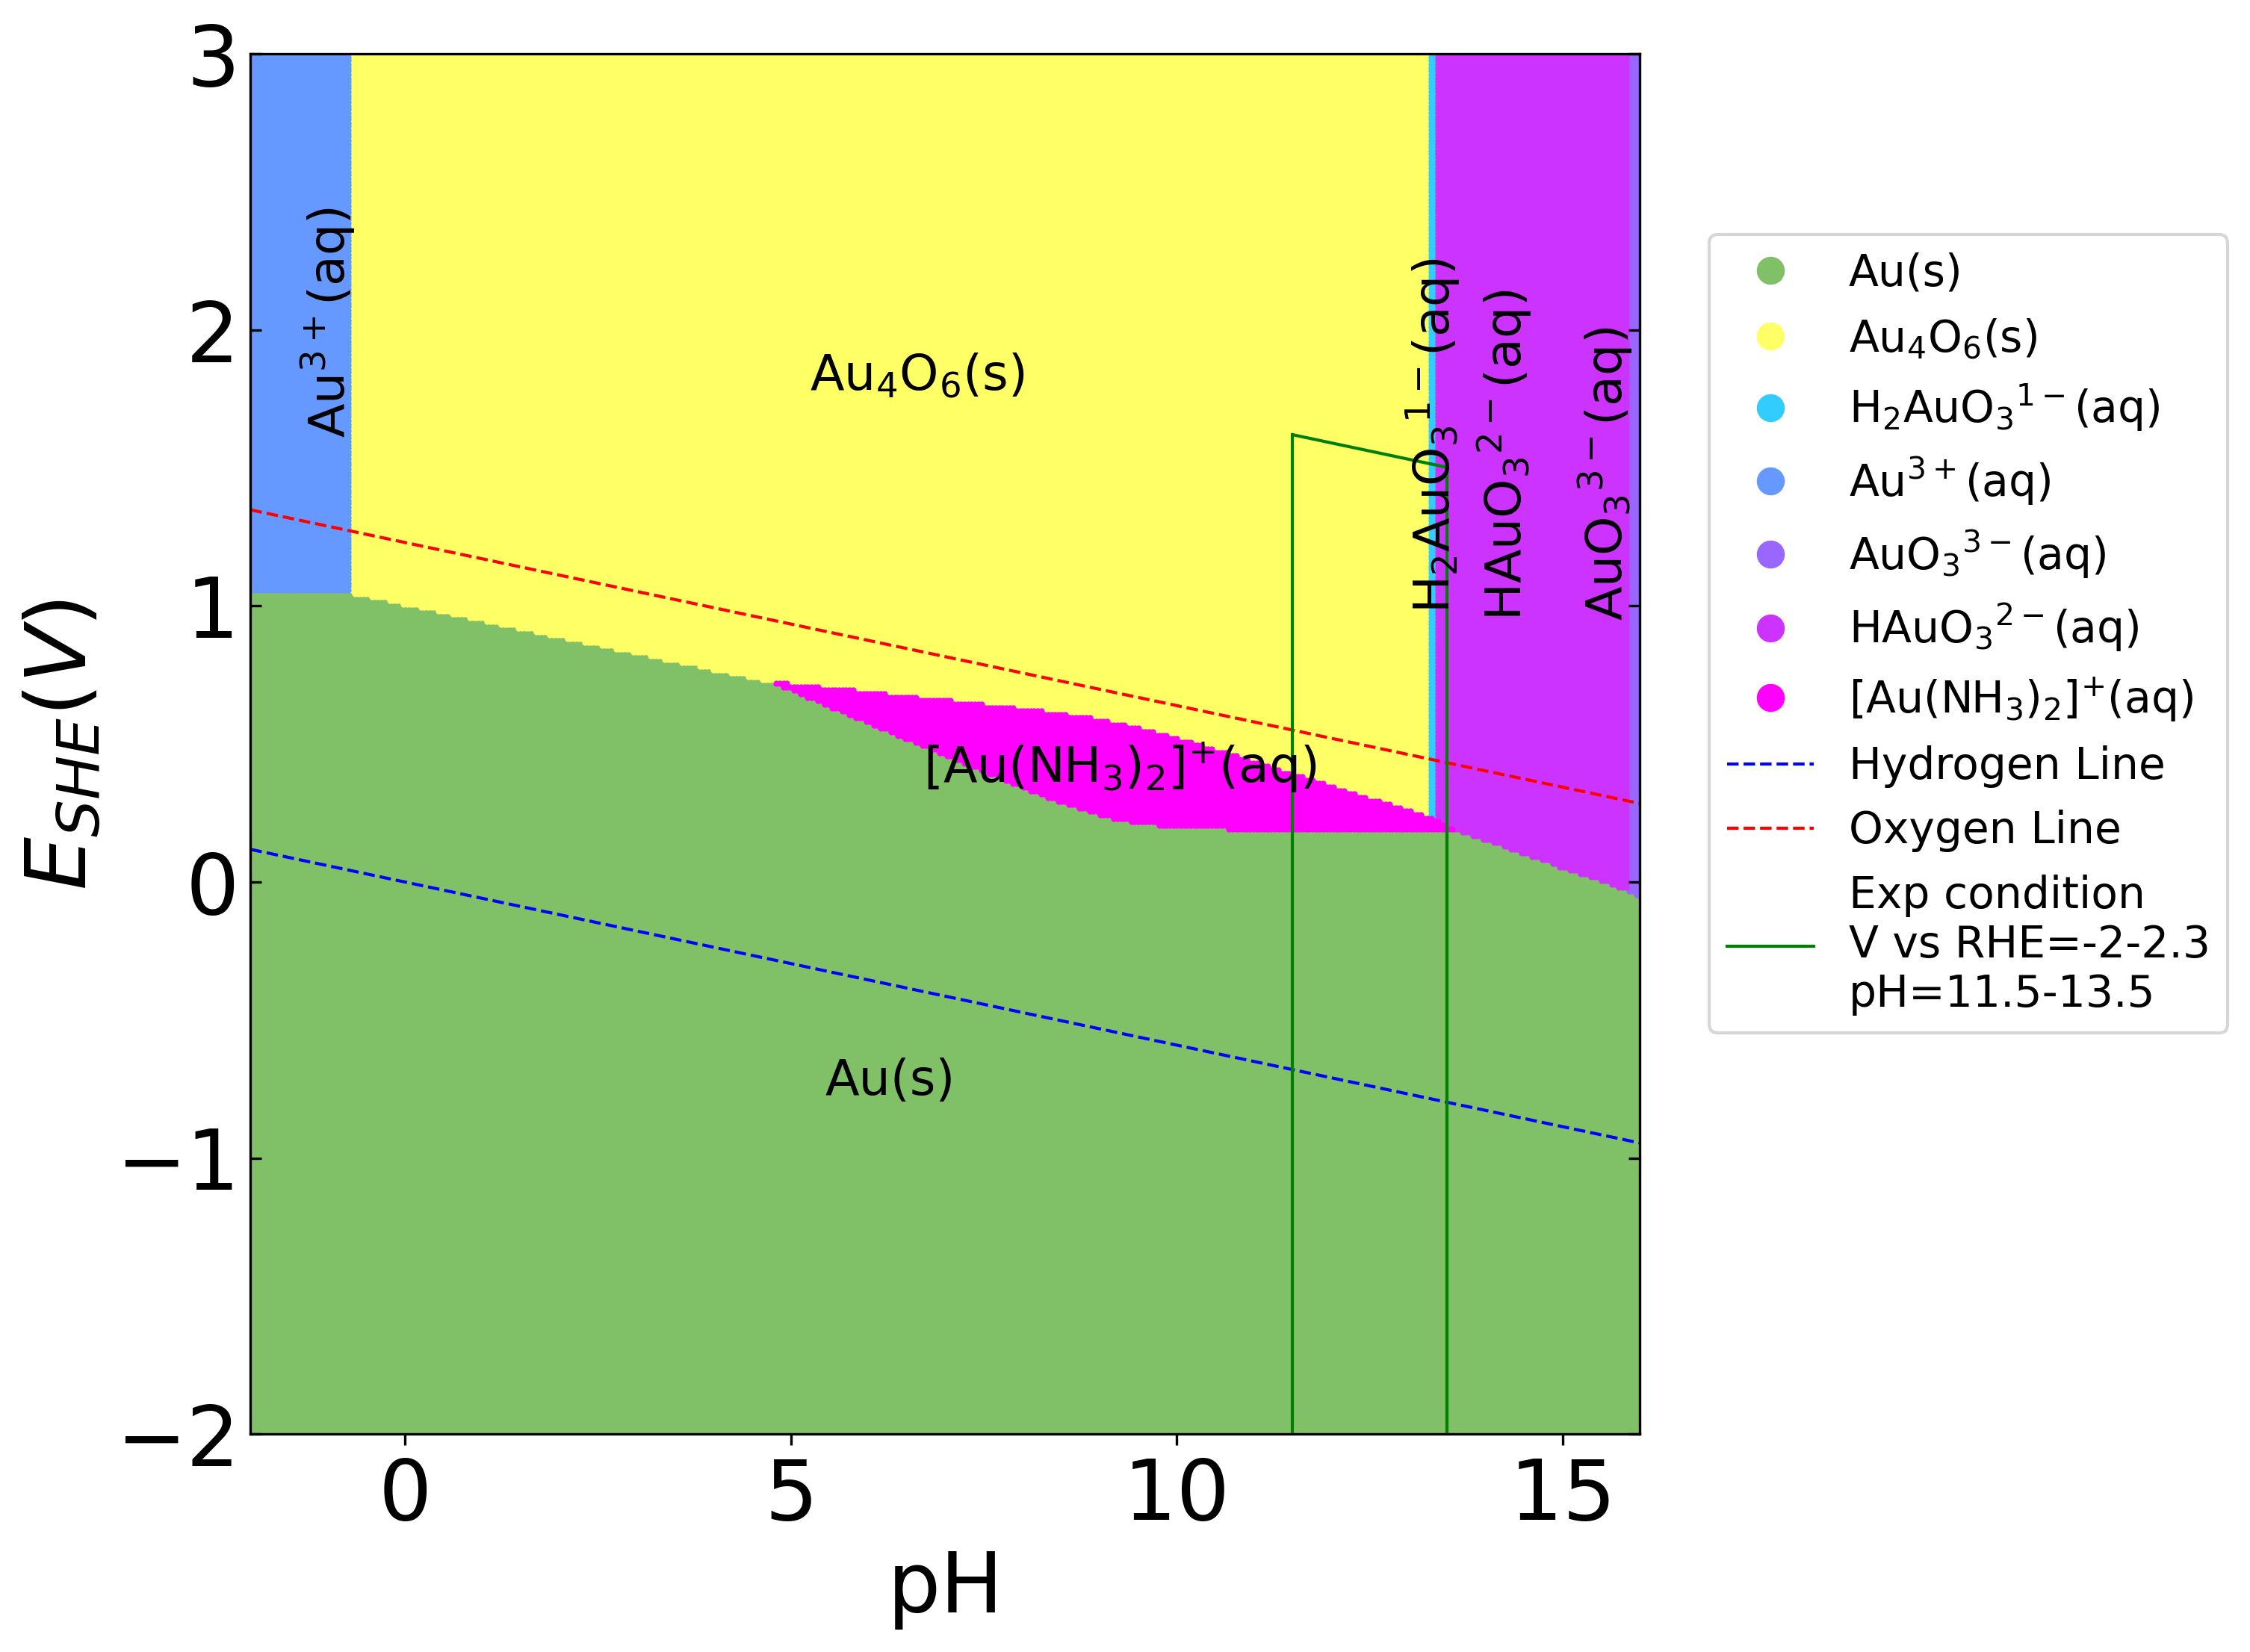
\includegraphics[width=0.5\textwidth]{Figures/pourbaix_diagrams/Au-NH3-H2O_activity=1e-04_[NH3]=0.02M_[Gly]=0.005M_[CN]=0.png}
%   \caption{Ni Pourbaix diagram at $[NH_3]_{initial}= 0.02M$, $[Gly]_{initial}=0.005M$. Green box indicates experimental condition at applied potential vs RHE = -2 to 2 V, pH =11.5 to 13.5}
%   \label{Au Pourbaix diagram}
% \end{figure}

% \begin{figure}
% 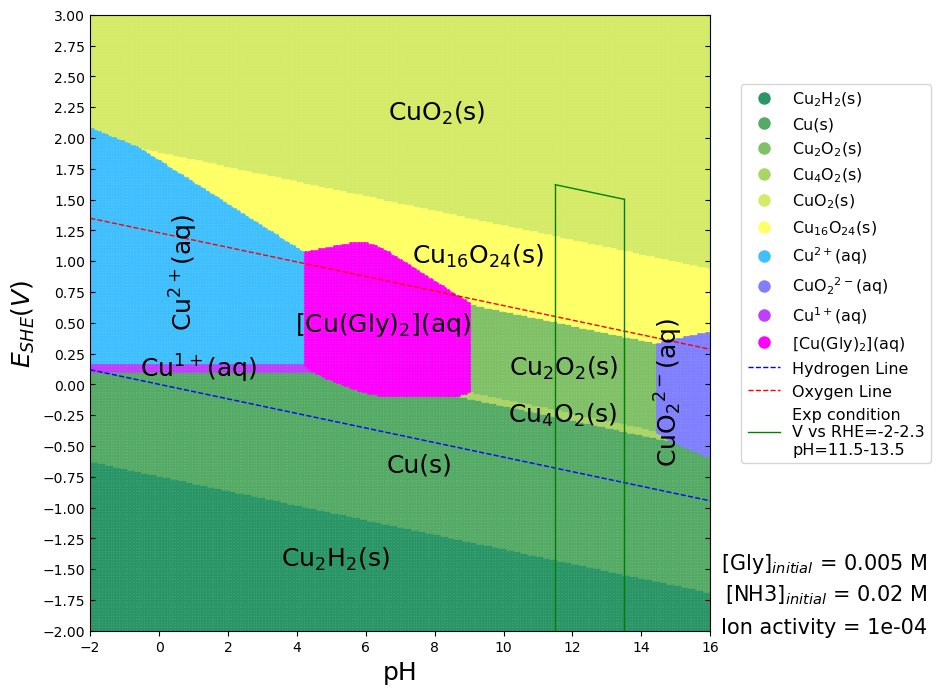
\includegraphics[width=0.5\textwidth]{Figures/pourbaix_diagrams/Cu-NH3-H2O_activity=1e-04_[NH3]=0.02M_[Gly]=0.005M_[CN]=0.png}
%   \caption{Ni Pourbaix diagram at $[NH_3]_{initial}= 0.02M$, $[Gly]_{initial}=0.005M$. Green box indicates experimental condition at applied potential vs RHE = -2 to 2 V, pH =11.5 to 13.5}
%   \label{Cu Pourbaix diagram}
% \end{figure}

% \begin{figure}
% 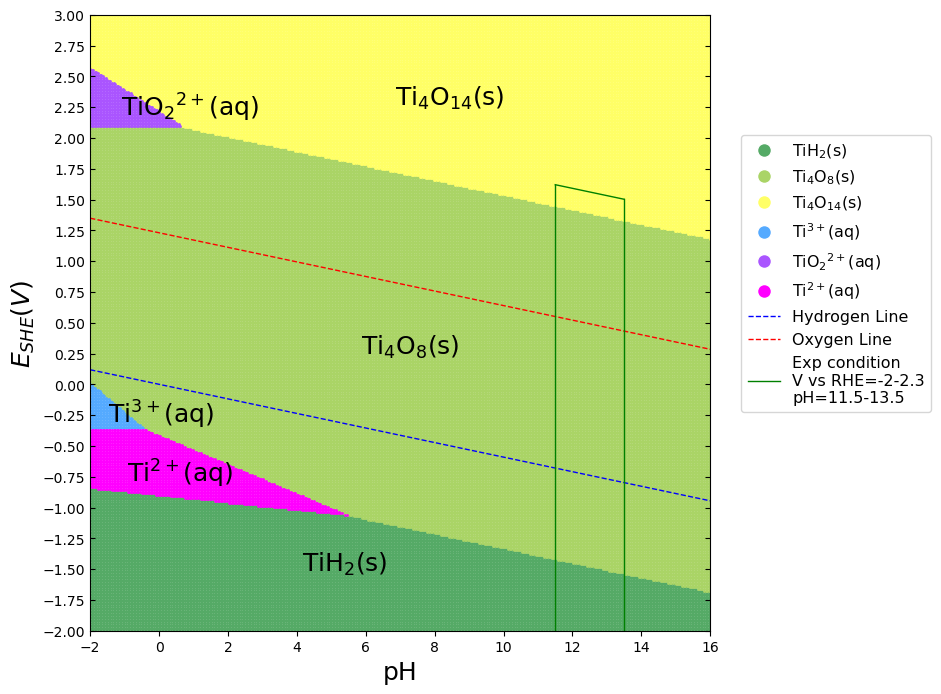
\includegraphics[width=0.5\textwidth]{Figures/pourbaix_diagrams/Ti-NH3-H2O_activity=1e-04_[NH3]=0.02M_[Gly]=0.005M_[CN]=0.png}
%   \caption{Ni Pourbaix diagram at $[NH_3]_{initial}= 0.02M$, $[Gly]_{initial}=0.005M$. Green box indicates experimental condition at applied potential vs RHE = -2 to 2 V, pH =11.5 to 13.5}
%   \label{Ti Pourbaix diagram}
% \end{figure}

% \begin{figure}
% 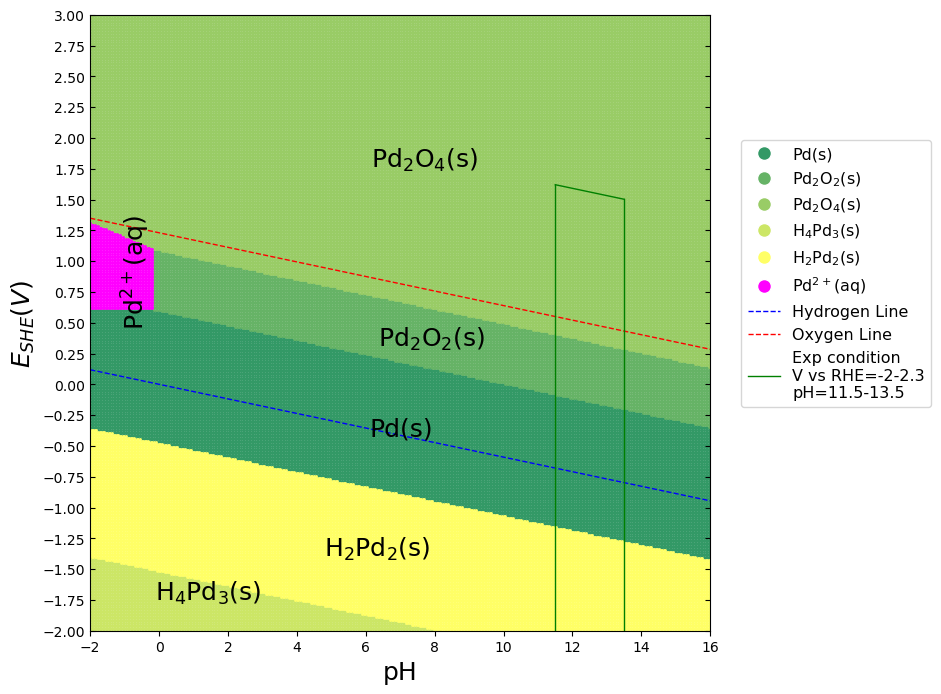
\includegraphics[width=0.5\textwidth]{Figures/pourbaix_diagrams/Pd-NH3-H2O_activity=1e-04_[NH3]=0.02M_[Gly]=0.005M_[CN]=0.png}
%   \caption{Ni Pourbaix diagram at $[NH_3]_{initial}= 0.02M$, $[Gly]_{initial}=0.005M$. Green box indicates experimental condition at applied potential vs RHE = -2 to 2 V, pH =11.5 to 13.5}
%   \label{Pd Pourbaix diagram}
% \end{figure}

% \begin{figure}
% 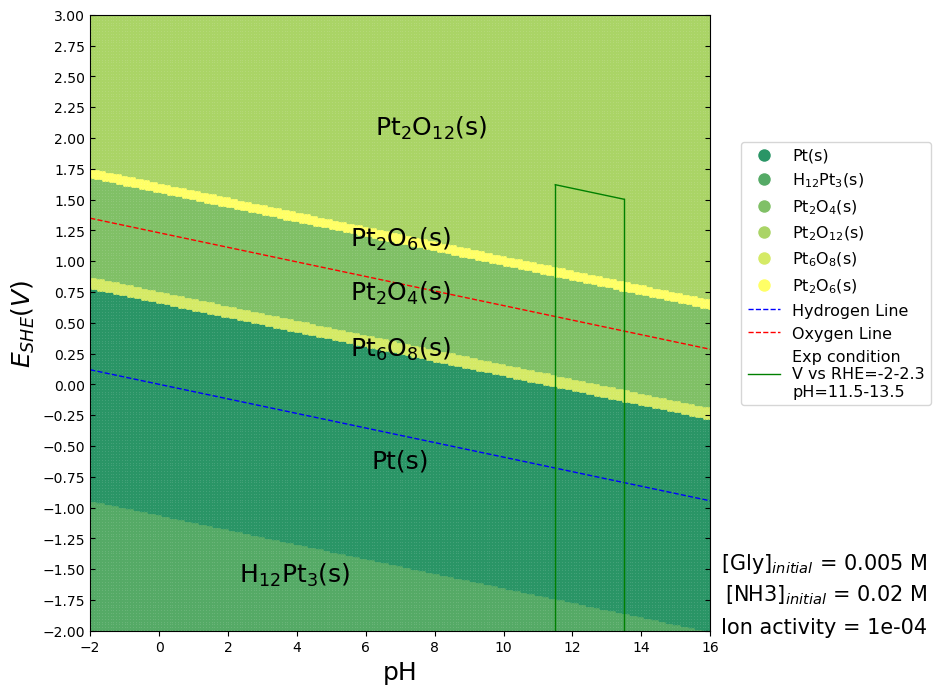
\includegraphics[width=0.5\textwidth]{Figures/pourbaix_diagrams/Pt-NH3-H2O_activity=1e-04_[NH3]=0.02M_[Gly]=0.005M_[CN]=0.png}
%   \caption{Ni Pourbaix diagram at $[NH_3]_{initial}= 0.02M$, $[Gly]_{initial}=0.005M$. Green box indicates experimental condition at applied potential vs RHE = -2 to 2 V, pH =11.5 to 13.5}
%   \label{Pt Pourbaix diagram}
% \end{figure}




\section{Conclusion}
Pourbaix diagrams of metal-\ce{NH3}/glycine/\ce{CN-}-\ce{H2O} are generated and discussed to identify thermodynamic behavior of an ideal material what can be used as an electrode in EWAS. The dissolvation behavior of various electrode under oxidizing potentials and high N-ligand concentrations was well explained by these pourbaix diagrams. The stability regions of build Ti and it oxides compared with other metals present its thermodynamically stability under such conditions. 
% \subsection{Outline}



% \subsection{References}

% The class makes various changes to the way that references are
% handled.  The class loads \textsf{natbib}, and also the
% appropriate bibliography style.  References can be made using
% the normal method; the citation should be placed before any
% punctuation, as the class will move it if using a superscript
% citation style
% \cite{Mena2000,Abernethy2003,Friedman-Hill2003,EuropeanCommission2008}.
% The use of \textsf{natbib} allows the use of the various citation
% commands of that package: \citeauthor{Abernethy2003} have shown
% something, in \citeyear{Cotton1999}, or as given by
% Ref.~\citenum{Mena2000}.  Long lists of authors will be
% automatically truncated in most article formats, but not in
% supplementary information or reviews \cite{Pople2003}. If you
% encounter problems with the citation macros, please check that
% your copy of \textsf{natbib} is up to date. The demonstration
% database file \texttt{achemso-demo.bib} shows how to complete
% entries correctly. Notice that ``\latin{et al.}'' is auto-formatted
% using the \texttt{\textbackslash latin} command.

% Multiple citations to be combined into a list can be given as
% a single citation.  This uses the \textsf{mciteplus} package
% \cite{Johnson1972,*Arduengo1992,*Eisenstein2005,*Arduengo1994}.
% Citations other than the first of the list should be indicated
% with a star. If the \textsf{mciteplus} package is not installed,
% the standard bibliography tools will still work but starred
% references will be ignored. Individual references can be referred
% to using \texttt{\textbackslash mciteSubRef}:
% ``ref.~\mciteSubRef{Eisenstein2005}''.

% The class also handles notes to be added to the bibliography.  These
% should be given in place in the document \bibnote{This is a note.
% The text will be moved the the references section.  The title of the
% section will change to ``Notes and References''.}.  As with
% citations, the text should be placed before punctuation.  A note is
% also generated if a citation has an optional note.  This assumes that
% the whole work has already been cited: odd numbering will result if
% this is not the case \cite[p.~1]{Cotton1999}.

% \subsection{Floats}

% New float types are automatically set up by the class file.  The
% means graphics are included as follows (Scheme~\ref{sch:example}).  As
% illustrated, the float is ``here'' if possible.
% \begin{scheme}
%   Your scheme graphic would go here: \texttt{.eps} format\\
%   for \LaTeX\, or \texttt{.pdf} (or \texttt{.png}) for pdf\LaTeX\\
%   \textsc{ChemDraw} files are best saved as \texttt{.eps} files:\\
%   these can be scaled without loss of quality, and can be\\
%   converted to \texttt{.pdf} files easily using \texttt{eps2pdf}.\\
%   %\includegraphics{graphic}
%   \caption{An example scheme}
%   \label{sch:example}
% \end{scheme}

% \begin{figure}
%   As well as the standard float types \texttt{table}\\
%   and \texttt{figure}, the class also recognises\\
%   \texttt{scheme}, \texttt{chart} and \texttt{graph}.
%   \caption{An example figure}
%   \label{fgr:example}
% \end{figure}

% Charts, figures and schemes do not necessarily have to be labelled or
% captioned.  However, tables should always have a title. It is
% possible to include a number and label for a graphic without any
% title, using an empty argument to the \texttt{\textbackslash caption}
% macro.

% The use of the different floating environments is not required, but
% it is intended to make document preparation easier for authors. In
% general, you should place your graphics where they make logical
% sense; the production process will move them if needed.

% \subsection{Math(s)}

% The \textsf{achemso} class does not load any particular additional
% support for mathematics.  If packages such as \textsf{amsmath} are
% required, they should be loaded in the preamble.  However,
% the basic \LaTeX\ math(s) input should work correctly without
% this.  Some inline material \( y = mx + c \) or $ 1 + 1 = 2 $
% followed by some display. \[ A = \pi r^2 \]

% It is possible to label equations in the usual way (Eq.~\ref{eqn:example}).
% \begin{equation}
%   \frac{\mathrm{d}}{\mathrm{d}x} \, r^2 = 2r \label{eqn:example}
% \end{equation}
% This can also be used to have equations containing graphical
% content. To align the equation number with the middle of the graphic,
% rather than the bottom, a minipage may be used.
% \begin{equation}
%   \begin{minipage}[c]{0.80\linewidth}
%     \centering
%     As illustrated here, the width of \\
%     the minipage needs to allow some  \\
%     space for the number to fit in to.
%     %\includegraphics{graphic}
%   \end{minipage}
%   \label{eqn:graphic}
% \end{equation}

% \section{Experimental}

% The usual experimental details should appear here.  This could
% include a table, which can be referenced as Table~\ref{tbl:example}.
% Notice that the caption is positioned at the top of the table.
% \begin{table}
%   \caption{An example table}
%   \label{tbl:example}
%   \begin{tabular}{ll}
%     \hline
%     Header one  & Header two  \\
%     \hline
%     Entry one   & Entry two   \\
%     Entry three & Entry four  \\
%     Entry five  & Entry five  \\
%     Entry seven & Entry eight \\
%     \hline
%   \end{tabular}
% \end{table}

% Adding notes to tables can be complicated.  Perhaps the easiest
% method is to generate these using the basic
% \texttt{\textbackslash textsuperscript} and
% \texttt{\textbackslash emph} macros, as illustrated (Table~\ref{tbl:notes}).
% \begin{table}
%   \caption{A table with notes}
%   \label{tbl:notes}
%   \begin{tabular}{ll}
%     \hline
%     Header one                            & Header two \\
%     \hline
%     Entry one\textsuperscript{\emph{a}}   & Entry two  \\
%     Entry three\textsuperscript{\emph{b}} & Entry four \\
%     \hline
%   \end{tabular}

%   \textsuperscript{\emph{a}} Some text;
%   \textsuperscript{\emph{b}} Some more text.
% \end{table}

% The example file also loads the optional \textsf{mhchem} package, so
% that formulas are easy to input: \texttt{\textbackslash ce\{H2SO4\}}
% gives \ce{H2SO4}.  See the use in the bibliography file (when using
% titles in the references section).

% The use of new commands should be limited to simple things which will
% not interfere with the production process.  For example,
% \texttt{\textbackslash mycommand} has been defined in this example,
% to give italic, mono-spaced text: \mycommand{some text}.



%%%%%%%%%%%%%%%%%%%%%%%%%%%%%%%%%%%%%%%%%%%%%%%%%%%%%%%%%%%%%%%%%%%%%
%% The "Acknowledgement" section can be given in all manuscript
%% classes.  This should be given within the "acknowledgement"
%% environment, which will make the correct section or running title.
%%%%%%%%%%%%%%%%%%%%%%%%%%%%%%%%%%%%%%%%%%%%%%%%%%%%%%%%%%%%%%%%%%%%%
\begin{acknowledgement}

% Please use ``The authors thank \ldots'' rather than ``The
% authors would like to thank \ldots''.

% The author thanks Mats Dahlgren for version one of \textsf{achemso},
% and Donald Arseneau for the code taken from \textsf{cite} to move
% citations after punctuation. Many users have provided feedback on the
% class, which is reflected in all of the different demonstrations
% shown in this document.

\end{acknowledgement}

%%%%%%%%%%%%%%%%%%%%%%%%%%%%%%%%%%%%%%%%%%%%%%%%%%%%%%%%%%%%%%%%%%%%%
%% The same is true for Supporting Information, which should use the
%% suppinfo environment.
%%%%%%%%%%%%%%%%%%%%%%%%%%%%%%%%%%%%%%%%%%%%%%%%%%%%%%%%%%%%%%%%%%%%%
\begin{suppinfo}
Free energies of metal-ligand complexes are available.


\end{suppinfo}

%%%%%%%%%%%%%%%%%%%%%%%%%%%%%%%%%%%%%%%%%%%%%%%%%%%%%%%%%%%%%%%%%%%%%
%% The appropriate \bibliography command should be placed here.
%% Notice that the class file automatically sets \bibliographystyle
%% and also names the section correctly.
%%%%%%%%%%%%%%%%%%%%%%%%%%%%%%%%%%%%%%%%%%%%%%%%%%%%%%%%%%%%%%%%%%%%%
\bibliography{references_mendeley_pourbaix}

\end{document}